\bookchapter{Bab 49: Membina Persekitaran Pembangunan — Android Studio dan Projek Pertama}

\chapterintro{Ingin membuat kerja dengan baik, tajamkan dahulu peralatan anda. Dalam bab ini kita 'memasang dapur': memasang Android Studio, menjayakan emulator, mencipta projek Android pertama dalam hidup anda, kemudian membongkar struktur projek untuk difahami dengan jelas. Selepas persekitaran siap dipasang, anda buat pertama kalinya akan melihat kod yang anda tulis bertukar menjadi butang yang boleh ditekan — detik ini, ramai orang ingat seumur hidup.}

\booksection{Memasang Android Studio}

Android Studio ialah persekitaran pembangunan bersepadu (IDE) rasmi Google, percuma, dengan pakej fungsi lengkap: menulis kod, melihat pratonton antara muka, menyahpepijat, membungkus — semuanya di dalamnya. Empat langkah pemasangan:

\begin{enumerate}
  \item Buka laman rasmi developer.android.com/studio dan muat turun versi stabil terkini (pada Ogos 2026, versi selepas Narwhal; ada untuk Windows/Mac/Linux);
  \item Jalankan pemasang, klik 'Seterusnya' dari mula hingga akhir — pembimbing pemasangan akan membawa Android SDK dan komponen emulator secara automatik;
  \item Semasa dilancarkan buat kali pertama, muat turun komponen SDK mengikut arahan (cukup guna pilihan lalai; mungkin mengambil masa beberapa minit dan beberapa GB ruang);
  \item Selepas selesai, anda akan melihat halaman alu-aluan — tahniah, 'dapur' sudah siap.
\end{enumerate}

\begin{tcbwarn}{Perhatian: Fahami Keperluan Perkakasan}
Android Studio ialah 'pemakan memori': disyorkan sekurang-kurangnya 16GB RAM (8GB pun boleh berjalan, tetapi emulator agak tersekat apabila dibuka), sediakan ruang cakera melebihi 20GB, dan CPU mesti menyokong virtualisasi (aktifkan VT-x/AMD-V dalam BIOS). Jika komputer anda memang tua, boleh guna 'penyahpepijatan peranti sebenar' sebagai ganti emulator (diterangkan dalam Bahagian 4 bab ini); pengalamannya malah lebih lancar.

\end{tcbwarn}

\booksection{Mencipta Projek Pertama Anda}

Di halaman alu-aluan, klik New Project, pilih templat Empty Activity (templat paling bersih untuk pemula), kemudian isi tiga perkara:

\begin{center}
\begin{tabularx}{\linewidth}{|X|X|X|}
\hline
\textbf{Item konfigurasi} & \textbf{Apa diisi} & \textbf{Penerangan} \tabularnewline
\hline
Name & My First App & Nama aplikasi, dipaparkan pada skrin utama telefon \tabularnewline
Package name & com.example.myfirstapp & Pengenal unik sejagat; lazimnya 'domain terbalik', ikut lalai dahulu \tabularnewline
Minimum SDK & API 26(Android 8.0) & Versi sokongan minimum, meliputi 95\%+ peranti \tabularnewline
\hline
\end{tabularx}
\end{center}

\begin{center}\small\color{gray}Tiga perkara yang perlu diisi semasa mencipta projek\end{center}

Selepas klik Finish, Android Studio akan memuat turun kebergantungan dan membina projek secara automatik dengan Gradle (kali pertama perlu menunggu beberapa minit; selepas itu jauh lebih pantas). Setelah siap dibina, anda mempunyai apl yang boleh berjalan — walaupun ia buat sementara hanya memaparkan satu baris “Hello Android!”.

\begin{tcbinfo}{Petua: Selok-belok Nama Pakej}
Nama pakej (package name) seperti 'nombor kad pengenalan' aplikasi; tidak boleh berulang di seluruh dunia, dan tidak boleh diubah selepas diterbitkan. Untuk latihan peribadi, com.example.xxx sudah memadai; produk sebenar mesti diganti dengan domain terbalik anda sendiri (contohnya com.nama.anda.namaaplikasi). Jangan terbitkan dengan com.example — kedai akan menolaknya.

\end{tcbinfo}

\booksection{Menjalankannya: Emulator dan Peranti Sebenar}

Kod sudah siap ditulis, kena cari 'telefon' untuk menjalankannya. Anda ada dua pilihan:

\booksubsection{Emulator}

Emulator ialah telefon Android yang dimayakan di dalam komputer. Dalam Android Studio, buka Device Manager Create Device, pilih satu peranti (disyorkan siri Pixel) pilih satu imej sistem (yang membawa Google APIs) muat turun mula. Kemudian tekan segi tiga hijau Run pada bar alat; beberapa saat kemudian, apl anda akan muncul pada skrin 'telefon' itu.

\booksubsection{Penyahpepijatan peranti sebenar (lebih disyorkan)}

Peranti sebenar sentiasa menjadi persekitaran ujian paling sebenar — rasa geseran semasa meluncur, rangkaian sebenar, sensor sebenar; emulator tidak dapat menandinginya. Penyahpepijatan peranti Android sebenar sangat mudah:

\begin{enumerate}
  \item Pada telefon, buka [Tetapan] [Mengenai Telefon], ketik 'Nombor Binaan' 7 kali berturut-turut untuk mengaktifkan 'Pilihan Pembangun';
  \item Dalam [Pilihan Pembangun], aktifkan Penyahpepijatan USB;
  \item Sambungkan telefon ke komputer dengan kabel data, dan pada tetingkap timbul telefon pilih 'Benarkan penyahpepijatan USB';
  \item Kembali ke Android Studio; telefon anda akan muncul dalam senarai juntai bawah peranti pada bar alat, kemudian tekan Run.
\end{enumerate}

\textbf{Amaran Perangkap: Jangan Biarkan Penyahpepijatan USB Sentiasa Aktif}\par

Penyahpepijatan USB umpama membuka 'pintu belakang' kepada komputer. Semasa mengecas di tempat awam atau menyambung kepada komputer yang tidak dipercayai, pastikan anda mematikan Penyahpepijatan USB untuk menghalang orang lain membaca data anda melaluinya. Matikan terus selepas selesai membangun — jadikan tabiat.

\booksection{Membongkar Struktur Projek: Apa Fungsi Setiap Fail}

Kali pertama membuka projek, pepohon fail di sebelah kiri mungkin membuatkan anda pening. Jangan panik; dalam pembangunan harian, 90\% masa anda hanya berurusan dengan beberapa yang berikut:

\begin{center}
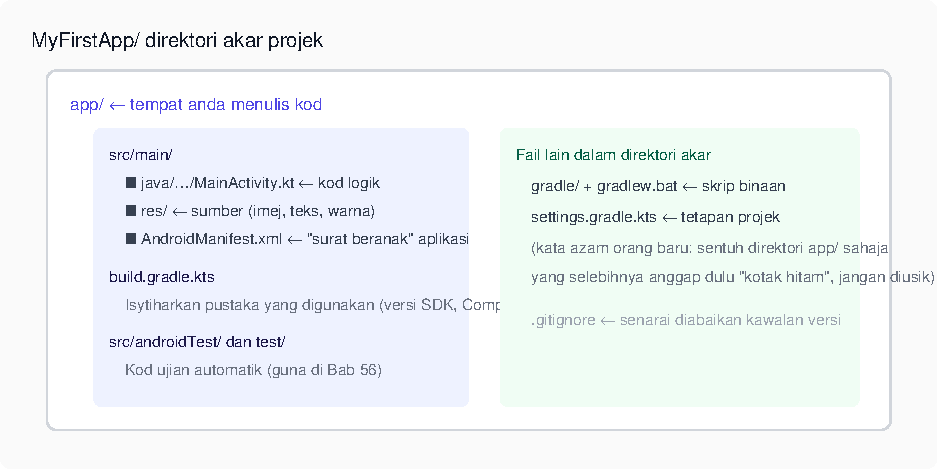
\includegraphics[width=0.92\linewidth]{figures/fig-di-si-shi-jiu-zhang-1}
\\[2pt]\small Rajah 2: Struktur projek yang wajib difahami pemula (rumus: sentuh hanya direktori app/)
\end{center}

\begin{itemize}
  \item MainActivity.kt: 'Pintu gerbang' aplikasi. Apabila pengguna mengetik ikon, inilah yang pertama dibangunkan. Dalam templat masa kini, ia bertanggungjawab memaparkan "Hello Android!".
  \item AndroidManifest.xml: 'Buku daftar' aplikasi — mengisytiharkan nama aplikasi ini, ikon yang mana, halaman apa yang ada, dan kebenaran apa yang diperlukan (kamera, lokasi dan sebagainya).
  \item Direktori res/: gudang sumber, menyimpan imej, ikon, rentetan, warna. Meletakkan teks dalam fail sumber dan bukannya menulis terus dalam kod ialah tabiat baik pembangunan Android (mudah untuk tukar bahasa, tukar tema).
  \item build.gradle.kts: resipi binaan — mengisytiharkan versi sokongan minimum dan pustaka kebergantungan (contohnya Compose).
\end{itemize}

\booksection{Uji Kemahiran: Gantikan 'Hello' dengan Nama Anda}

Buka MainActivity.kt dan anda akan melihat kod yang dijana oleh templat Compose. Cari baris Text(“Hello Android!”), gantikan teks dalam tanda petik dengan nama anda, contohnya Text(“Hai, Ali! Ini aplikasi pertama saya”), kemudian tekan Ctrl+R (Cmd+R pada Mac) untuk menjalankan semula. Beberapa saat kemudian, nama anda terpamer pada emulator.

\begin{lstlisting}[language=Kotlin]
setContent {
    MyFirstAppTheme {
        Surface(modifier = Modifier.fillMaxSize()) {
            // v Tukar bahagian ini kepada teks anda sendiri
            Text("Hai, Zhang San! Ini aplikasi pertama saya")
        }
    }
}
\end{lstlisting}

Tahniah, anda telah melengkapkan satu kitaran penuh 'ubah kod bina pasang jalankan'. Kitaran inilah rutin pembangunan harian anda pada masa hadapan. Sementara masih hangat, cuba ubah sesuatu yang lain: besarkan saiz fon, tukar warna — bab seterusnya kita akan belajar bagaimana 'sihir' ini datang.

\booksection{Pertolongan Cemas Ralat Biasa: 'Bilik Kecemasan' Dua Minggu Pertama Pemula}

Pada peringkat penyediaan persekitaran dan binaan pertama, anda berkemungkinan besar menghadapi tiga ralat berikut. Jangan panik; semuanya ada penawar:

\begin{center}
\begin{tabularx}{\linewidth}{|X|X|X|}
\hline
\textbf{Gejala ralat} & \textbf{Punca biasa} & \textbf{Penawar} \tabularnewline
\hline
Gradle sync failed / muat turun kebergantungan lambat & Akses rangkaian ke repositori tidak lancar & Konfigurasikan repositori cermin tempatan untuk Gradle (cermin maven Aliyun/Tencent Cloud), cari 'gradle mirror tempatan' di internet dan ubah mengikut arahan \tabularnewline
Komponen SDK tidak lengkap & Muat turun SDK dilangkau semasa pemasangan & Settings SDK Manager untuk memasang platform dan alat yang kurang \tabularnewline
Emulator gagal dimulakan / skrin hitam & Virtualisasi tidak diaktifkan; imej rosak & Aktifkan VT-x/AMD-V dalam BIOS; padam emulator dan bina semula; atau guna terus penyahpepijatan peranti sebenar \tabularnewline
\hline
\end{tabularx}
\end{center}

\begin{center}\small\color{gray}Jadual pertolongan cemas ralat persekitaran untuk pemula\end{center}

\begin{tcbinfo}{Petua: Metodologi Mencari Ralat}
Baris pertama mesej ralat paling bernilai — salinkan apa adanya ke dalam enjin carian, tambah kata kunci “android studio”. Jangan cari soalan umum seperti “kenapa saya tidak boleh pasang persekitaran”, cari ralat spesifik seperti “Gradle sync failed: Could not resolve com.android.tools.build”. Soalan yang tepat barulah menghasilkan jawapan yang tepat.

\end{tcbinfo}

\begin{tcbpractice}{Mari cuba: Lengkapkan senarai 'ritual pembangun' anda}
(1) Pasang Android Studio dan jayakan emulator; (2) jalankan aplikasi anda sekali pada peranti sebenar dan simpan tangkapan skrin sebagai kenangan; (3) ubah teks Hello kepada nama anda; (4) mampatkan projek sebagai arkib simpanan. Selepas melengkapkan empat langkah ini, anda boleh mengumumkan di media sosial: saya kini juga seorang pembangun Android (tangkapan skrin sebagai bukti).

\end{tcbpractice}

\begin{tcbsummary}{Ringkasan Bab}
\begin{itemize}
  \item Android Studio = IDE rasmi percuma; disyorkan 16GB RAM + 20GB cakera + aktifkan virtualisasi
  \item Tiga elemen projek baharu: nama, nama pakej (unik sejagat, jangan terbitkan dengan com.example), SDK minimum (mulai API 26)
  \item Dua cara menjalankan: emulator (telefon maya dalam komputer) dan peranti sebenar (aktifkan penyahpepijatan USB, ingat matikan selepas guna)
  \item Rumus projek: sentuh hanya direktori app/ — MainActivity.kt ialah pintu gerbang, Manifest ialah buku daftar, res/ ialah gudang sumber
  \item Rutin pembangunan = ubah kod Run lihat hasil, berulang-ulang
\end{itemize}

\end{tcbsummary}
